\documentclass[12pt]{article}
\usepackage[T2A]{fontenc}
\usepackage[utf8]{inputenc}
\usepackage{multirow}
\usepackage{caption}
\usepackage{subcaption}
\usepackage{amsmath}
\usepackage{changepage}
\usepackage{graphicx}
\usepackage{float}
\usepackage[english,russian]{babel}
\usepackage{amsmath, amsfonts, amssymb, amsthm, mathtools}
\usepackage{xcolor}
\usepackage{array}
\usepackage{hyperref}
\usepackage{icomma}
\usepackage{mathtext} 
\usepackage[top = 1.5cm, left = 1.5 cm, right = 1.5 cm, bottom = 3 cm]{geometry}
\graphicspath{ {./images/} }
 
\date{\today}
  
\begin{document}
\begin{titlepage}
	\begin{center}
		{\large МОСКОВСКИЙ ФИЗИКО-ТЕХНИЧЕСКИЙ ИНСТИТУТ (НАЦИОНАЛЬНЫЙ ИССЛЕДОВАТЕЛЬСКИЙ УНИВЕРСИТЕТ)}
	\end{center}
	\begin{center}
		{\large Физтех-школа физики и исследований им. Ландау}
	\end{center}

	\vspace{3cm}
	{\huge
		\begin{center}
			\textbf{Исследование самовозбуждающихся режимов работы схемы Чуа.}
		\end{center}
	}
	\vspace{2cm}
	\begin{flushright}
		{\LARGE Автор:\\ Шахматов Андрей Юрьевич \\
			\vspace{0.2cm}
			Б02-304}
	\end{flushright}
	\vspace{7 cm}
	\begin{center}
		Долгопрудный 2024
	\end{center}
	\thispagestyle{empty}
\end{titlepage}

% \maketitle

\begin{abstract}
	Надо написать.
\end{abstract}

% \tableofcontents

\section*{Введение}
В современном мире проблема обеспечения безопасности информации становится все более актуальной.
Одним из перспективных решений данной задачи является использование хаотических сигналов в качестве несущей волны.
Такой подход значительно повышает уровень защиты данных,
так как злоумышленник сталкивается с практически неразрешимой задачей расшифровки хаотического сигнала.

Для генерации хаотических сигналов широко применяется схема Чуа, включающая два конденсатора,
индуктивность, сопротивление и нелинейный элемент --- диод Чуа.
Простота конструкции делает эту схему привлекательной для различных отраслей промышленности.
Однако, несмотря на наличие теоретической модели, описывающей поведение схемы Чуа,
её практическое применение сталкивается с рядом сложностей, такими как высокая чувствительность контура и
ограниченная область хаотического поведения.

Целью данной работы является детальное исследование хаотических режимов работы схемы Чуа,
а также устойчивых нехаотических режимов, сосуществующих с хаотическими.

\section*{Теоретическая часть}
\subsection*{Хаотические системы}
тут нужна теоретическая справка про хаос

\subsection*{Устройство схемы Чуа}
\begin{figure}[H]
	\centering
	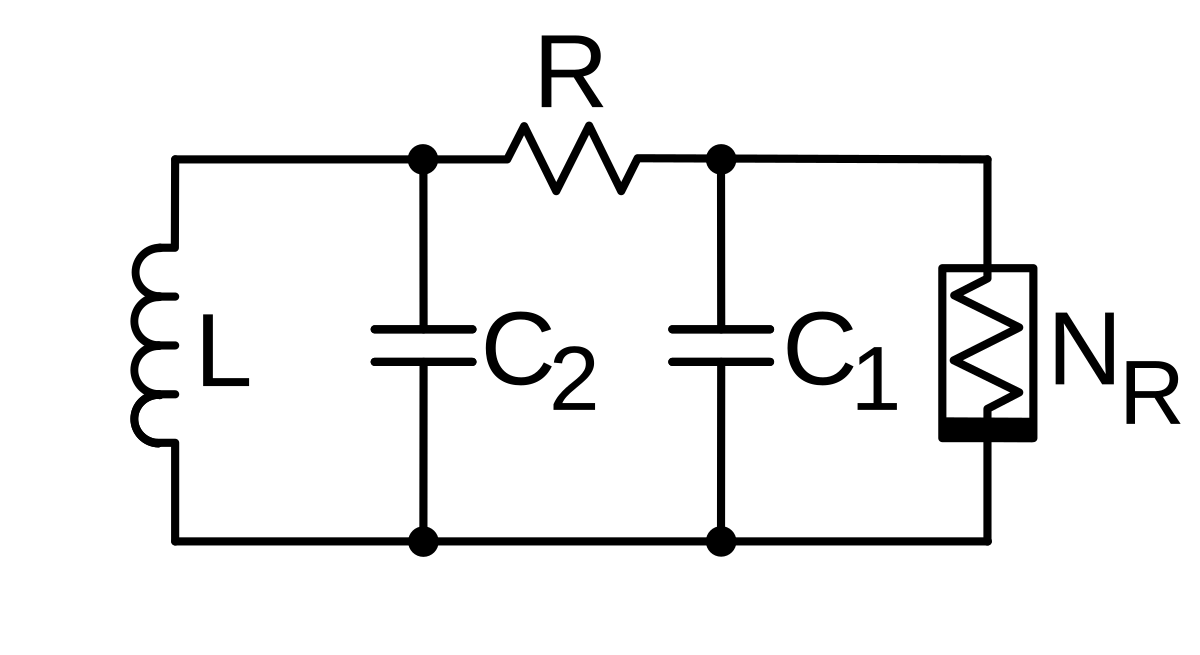
\includegraphics[width=0.4\textwidth]{Base_chua_curcuit.png}
	\hfil
	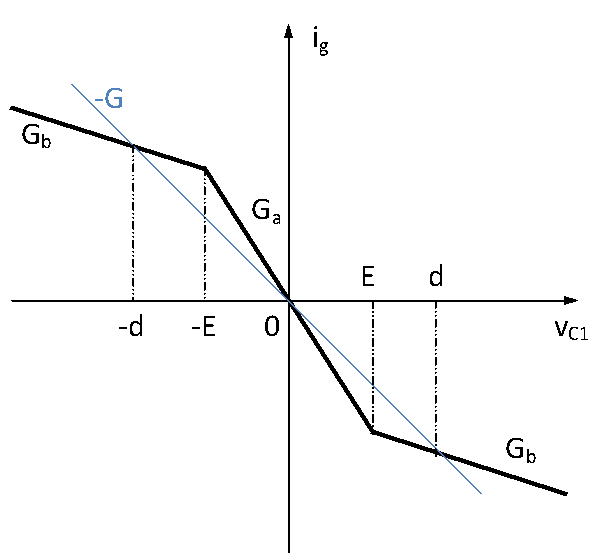
\includegraphics[width=0.35\textwidth]{chua_VAC.png}
	\caption{Электрическая схема цепи Чуа и вольт-амперная характеристика диода Чуа $N_R$.}
	\label{fig:base_curcuit}
\end{figure}
Классическая схема Чуа состоит из двух конденсаторов, сопротивления, индуктивности и диода Чуа.
Диод Чуа возможно реализовать при помощи использования двух операционных усилителей и шести резисторов (Рис. \ref{fig:OA_Gyrator}).
Также в реальности использование физической индуктивности может приводить к плохим результатам из-за наличия большого внутреннего
сопротивления. По этой причине в нашей работе индуктивность была заменена схемой на основе операционных усилителей --- гиратором (Рис. \ref{fig:OA_Gyrator}).
Эквивалентную индуктивность полученной схемы можно расчитать
\begin{eqnarray}
	L = \frac{R_7 R_9 R_{10} C}{R_8},
	\label{eq:gyrator}
\end{eqnarray}
где $R$ пронумерованы в порядке от врехнего к нижнему на схеме.

\begin{figure}[H]
	\centering
	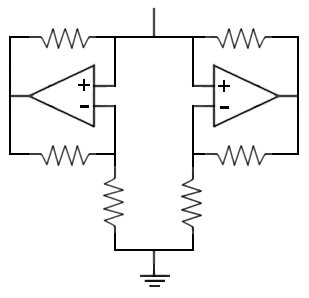
\includegraphics[width=0.35\textwidth]{OA.jpg}
	\hfil
	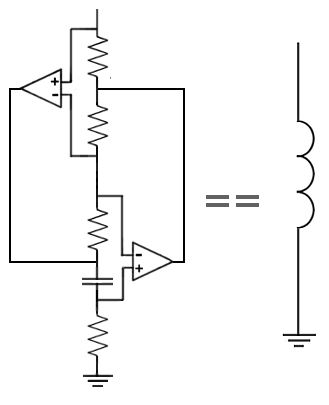
\includegraphics[width=0.35\textwidth]{gyrator.jpg}
	\caption{Реализация диода Чуа на основе операционных усилителей и эквивалентная индуктивности схема гиратора.}
	\label{fig:OA_Gyrator}
\end{figure}

Применяя полученные модификации получим исходную вариацию схемы с использованием только операционных усилителей, конденсаторов и сопротивлений (Рис. \ref{fig:final_curcuit}).
\begin{figure}[H]
	\centering
	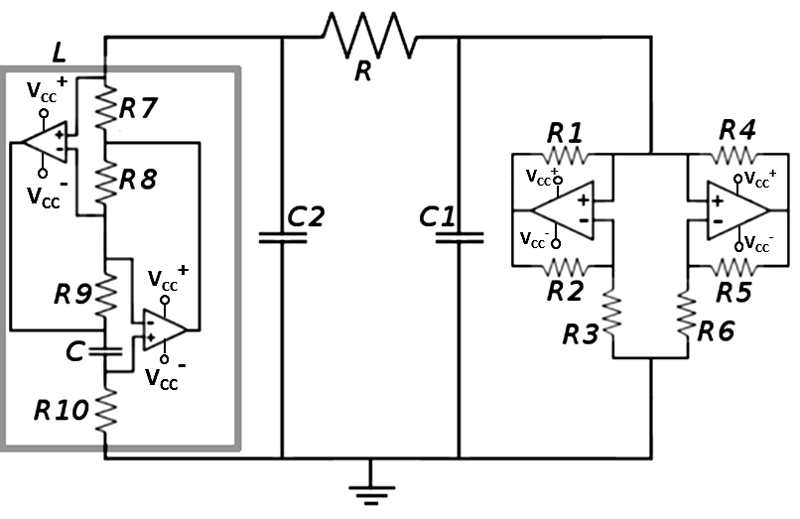
\includegraphics[width=0.55\textwidth]{chua_curcuit.jpg}
	\caption{Итоговая электрическая схема цепи Чуа, использующаяся в данной работе.}
	\label{fig:final_curcuit}
\end{figure}

Резисторы $R$ и $R_{10}$ являются переменными ползунковыми резисторами.
Точные характеристики элементов приведены в приложении (Таблица \ref{tab:curcuit_chars}).

\subsection*{Математическая модель схемы Чуа}
Обозначив за $U_{C_1}, U_{C_2}, I_{L}$ напряжения на конденсаторах и ток через катушку соответственно можно записать систему уравнений, описывающую цепь Чуа: 
\begin{equation}
	\begin{dcases}
		C_1 \frac{d U_{C_1}}{dt} = \frac{U_{C_2} - U_{C_1}}{R} - g(U_{C_1}), \\
		C_2 \frac{d U_{C_2}}{dt} = \frac{U_{C_1} - U_{C_2}}{R} + I_L, \\ 
		L \frac{d I_L}{dt} = -U_{C_2},
	\end{dcases}
	\label{eq:chua_system}
\end{equation} 
где $R$ --- сопротивление резистора, $L$ --- индуктивность катушки, $C_1, C_2$ --- ёмкости конденсаторов, а $g$ --- функция зависимости тока от напряжения 
на диоде Чуа: 
\[
	g(U_{C_1}) = G_b U_{C_1} + \frac{1}{2} \left( G_a - G_b \right) \left( \vert U_{C_1} + E \vert - \vert U_{C_1} - E \vert \right),
\]
где $G_b, G_a, E$ --- проводимости соответствующих участков и точки излома на рисунке \ref{fig:base_curcuit}.

Введя новые обозначения можно привести систему к новым безразмерным переменным: 
\[
	\begin{dcases}
		\frac{dx}{d \tau} = \alpha(y - x - h(x)), \\
		\frac{dy}{d \tau} = x - y + z, \\
		\frac{dz}{d \tau} = -\beta y, \\
	\end{dcases}
\]
где $m_0 = R G_a$, $m_1 = R G_b$, $\alpha = \frac{C_2}{C_1}$, $\beta = \frac{R^2 C_2}{L}$, 
$\tau = \frac{t}{R C_2}$, $x = \frac{U_{C_1}}{E}$, $y = \frac{U_{C_2}}{E}$, $z = \frac{I_L R}{E}$, и функция $h(x)$ равна 
\[
	h(x) = m_1 x + \frac{1}{2}(m_0 - m_1)(\vert x + 1 \vert - \vert x - 1 \vert ).
\]

\section*{Результаты и их анализ}
\subsection*{Численное моделирование}
Проведёно численное моделирование схемы Чуа с указанными в приложении параметрами, согласно дифференциальным уравнениям \ref{eq:chua_system}. 
Моделирование проводилось с шагом $\Delta R = 50$ Ом и $\Delta R_L = 150$ Ом. После моделирования получен набор 
изображений фазовых портретов системы при различных её параметрах \ref{fig:simulation}.
\begin{figure}[H]
	\centering
	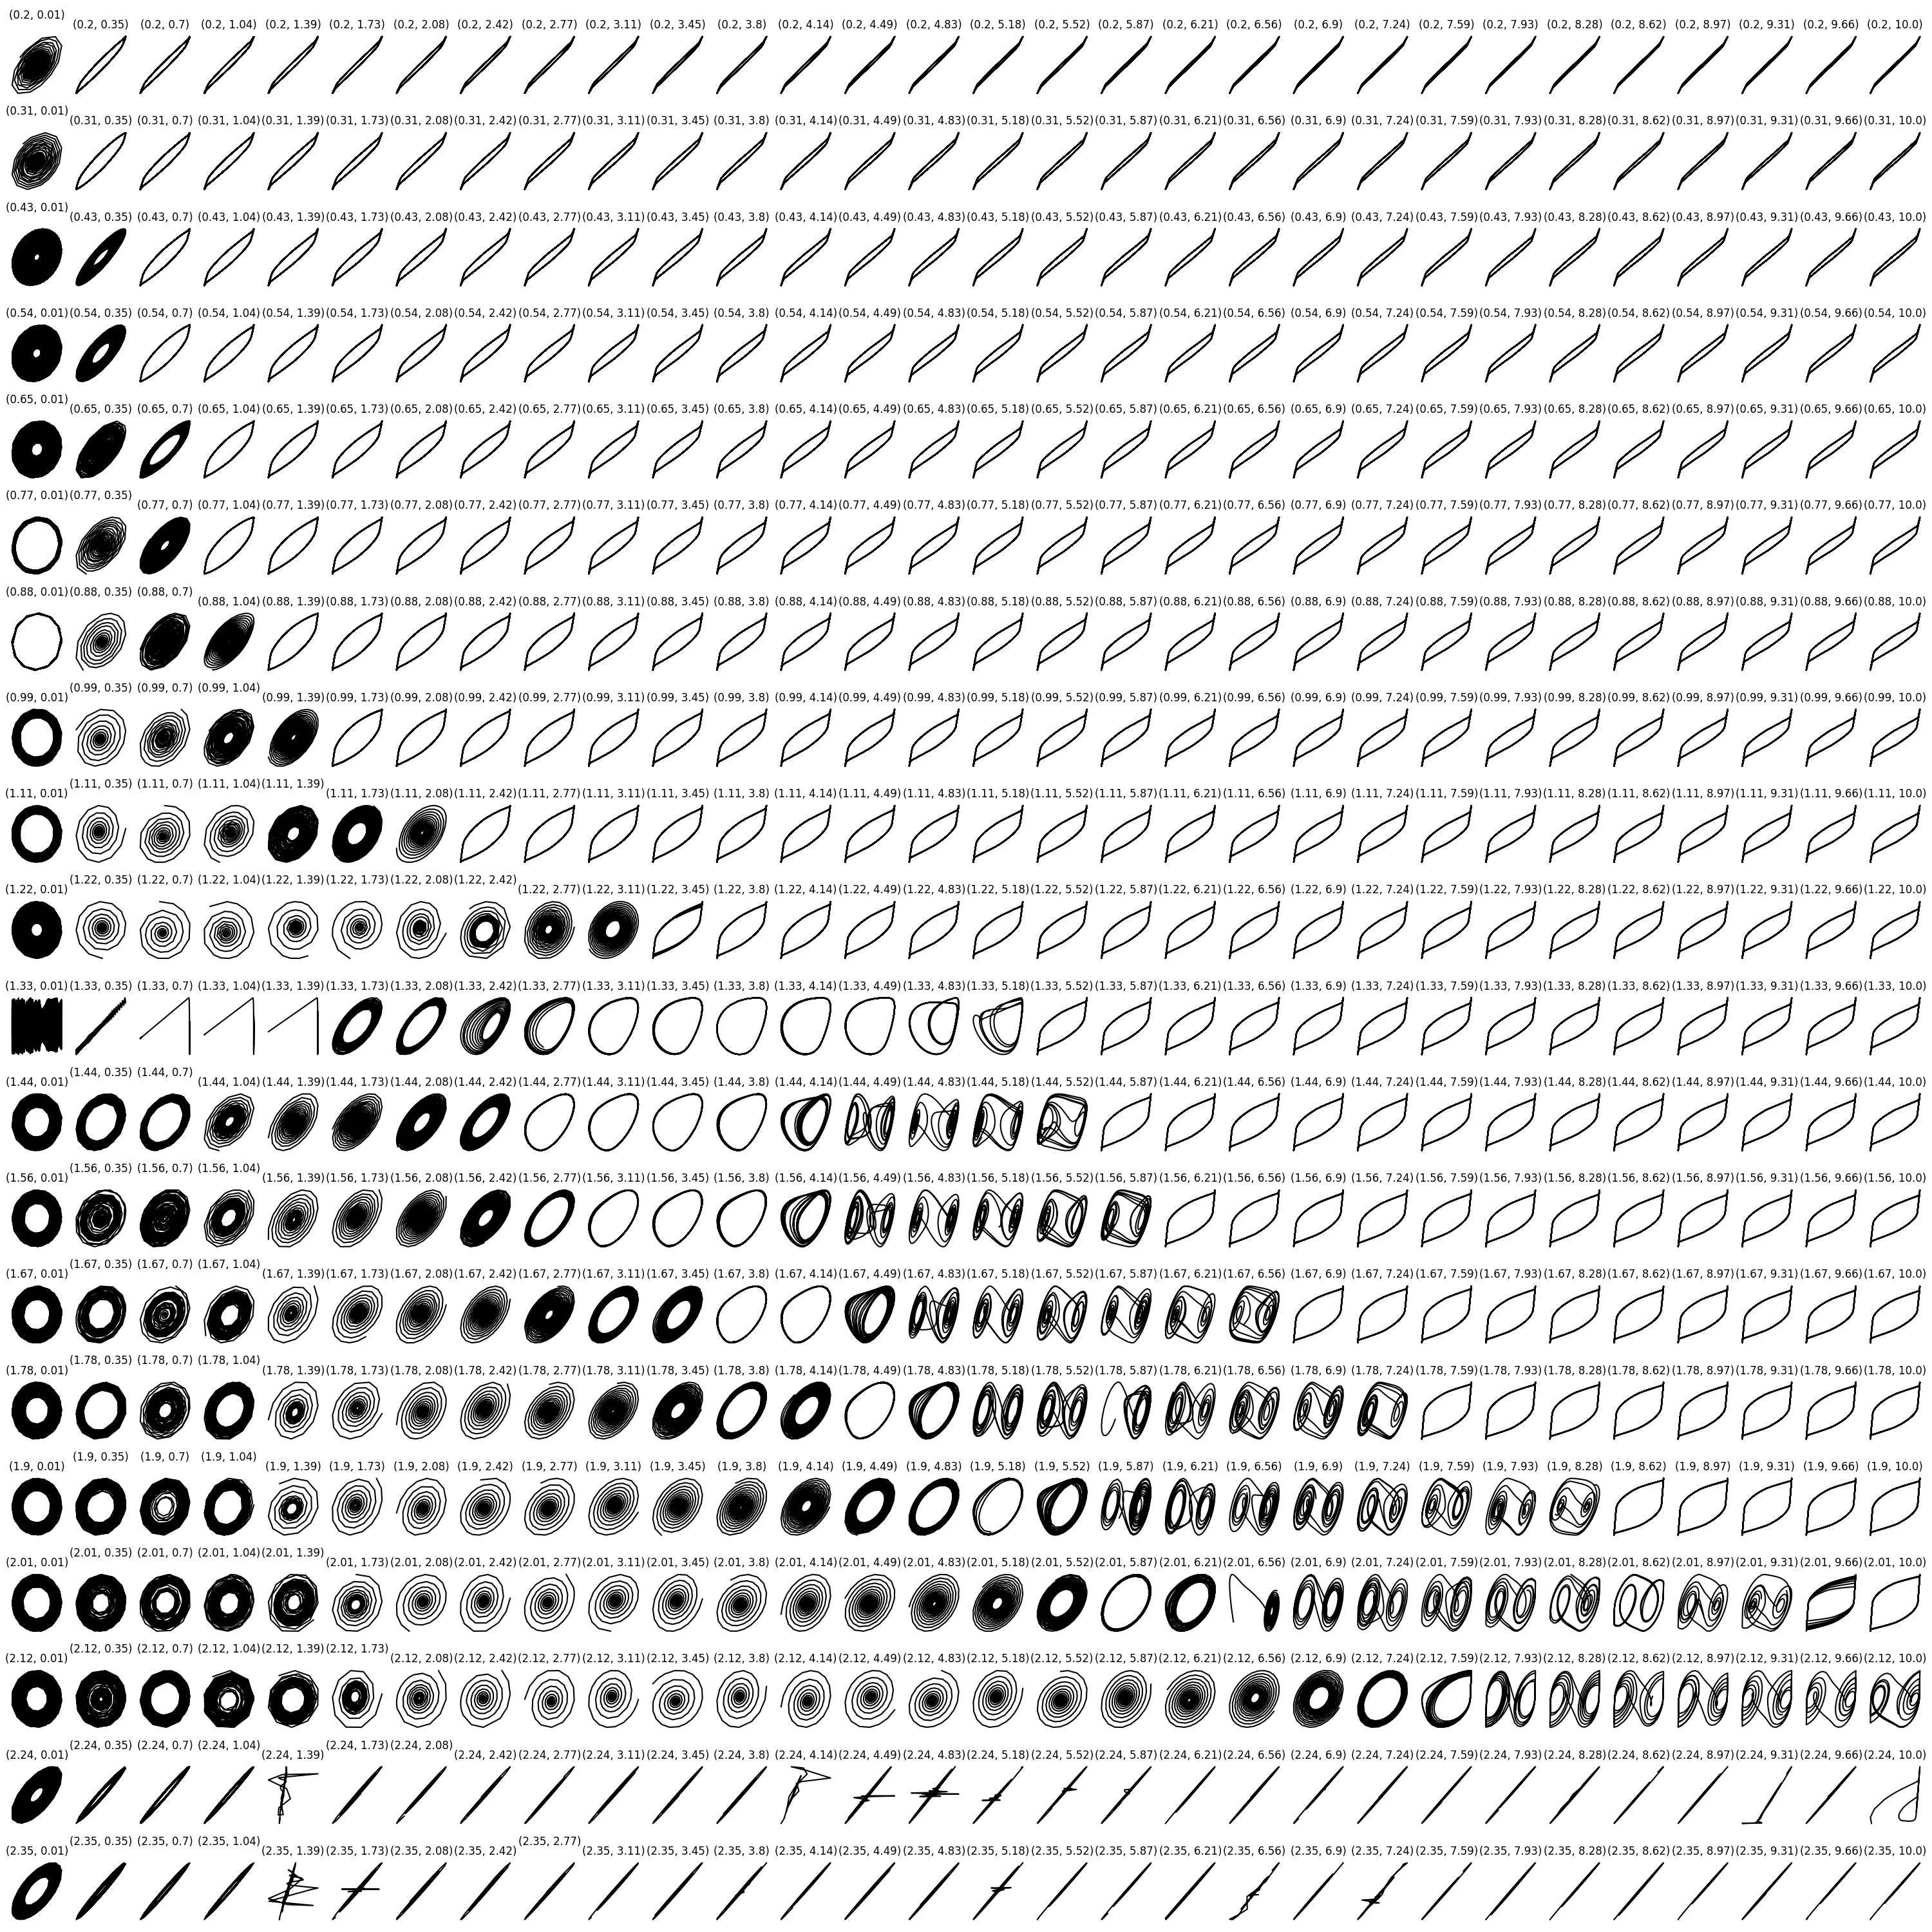
\includegraphics[width=0.55\textwidth]{sim_ex.png}
	\caption{Пример результата симуляции, полученной при $\Delta R = 110$ Ом и $\Delta R_L = 350$ Ом.}
	\label{fig:simulation}
\end{figure}
На полученной диаграмме можно выделить несколько областей с принципиально различными состояниями. 
По диаграмме определены пограничные кривые между различными состояниями системы и построен график \ref{fig:phase_diag_teor}. 

\begin{figure}[H]
	\centering
	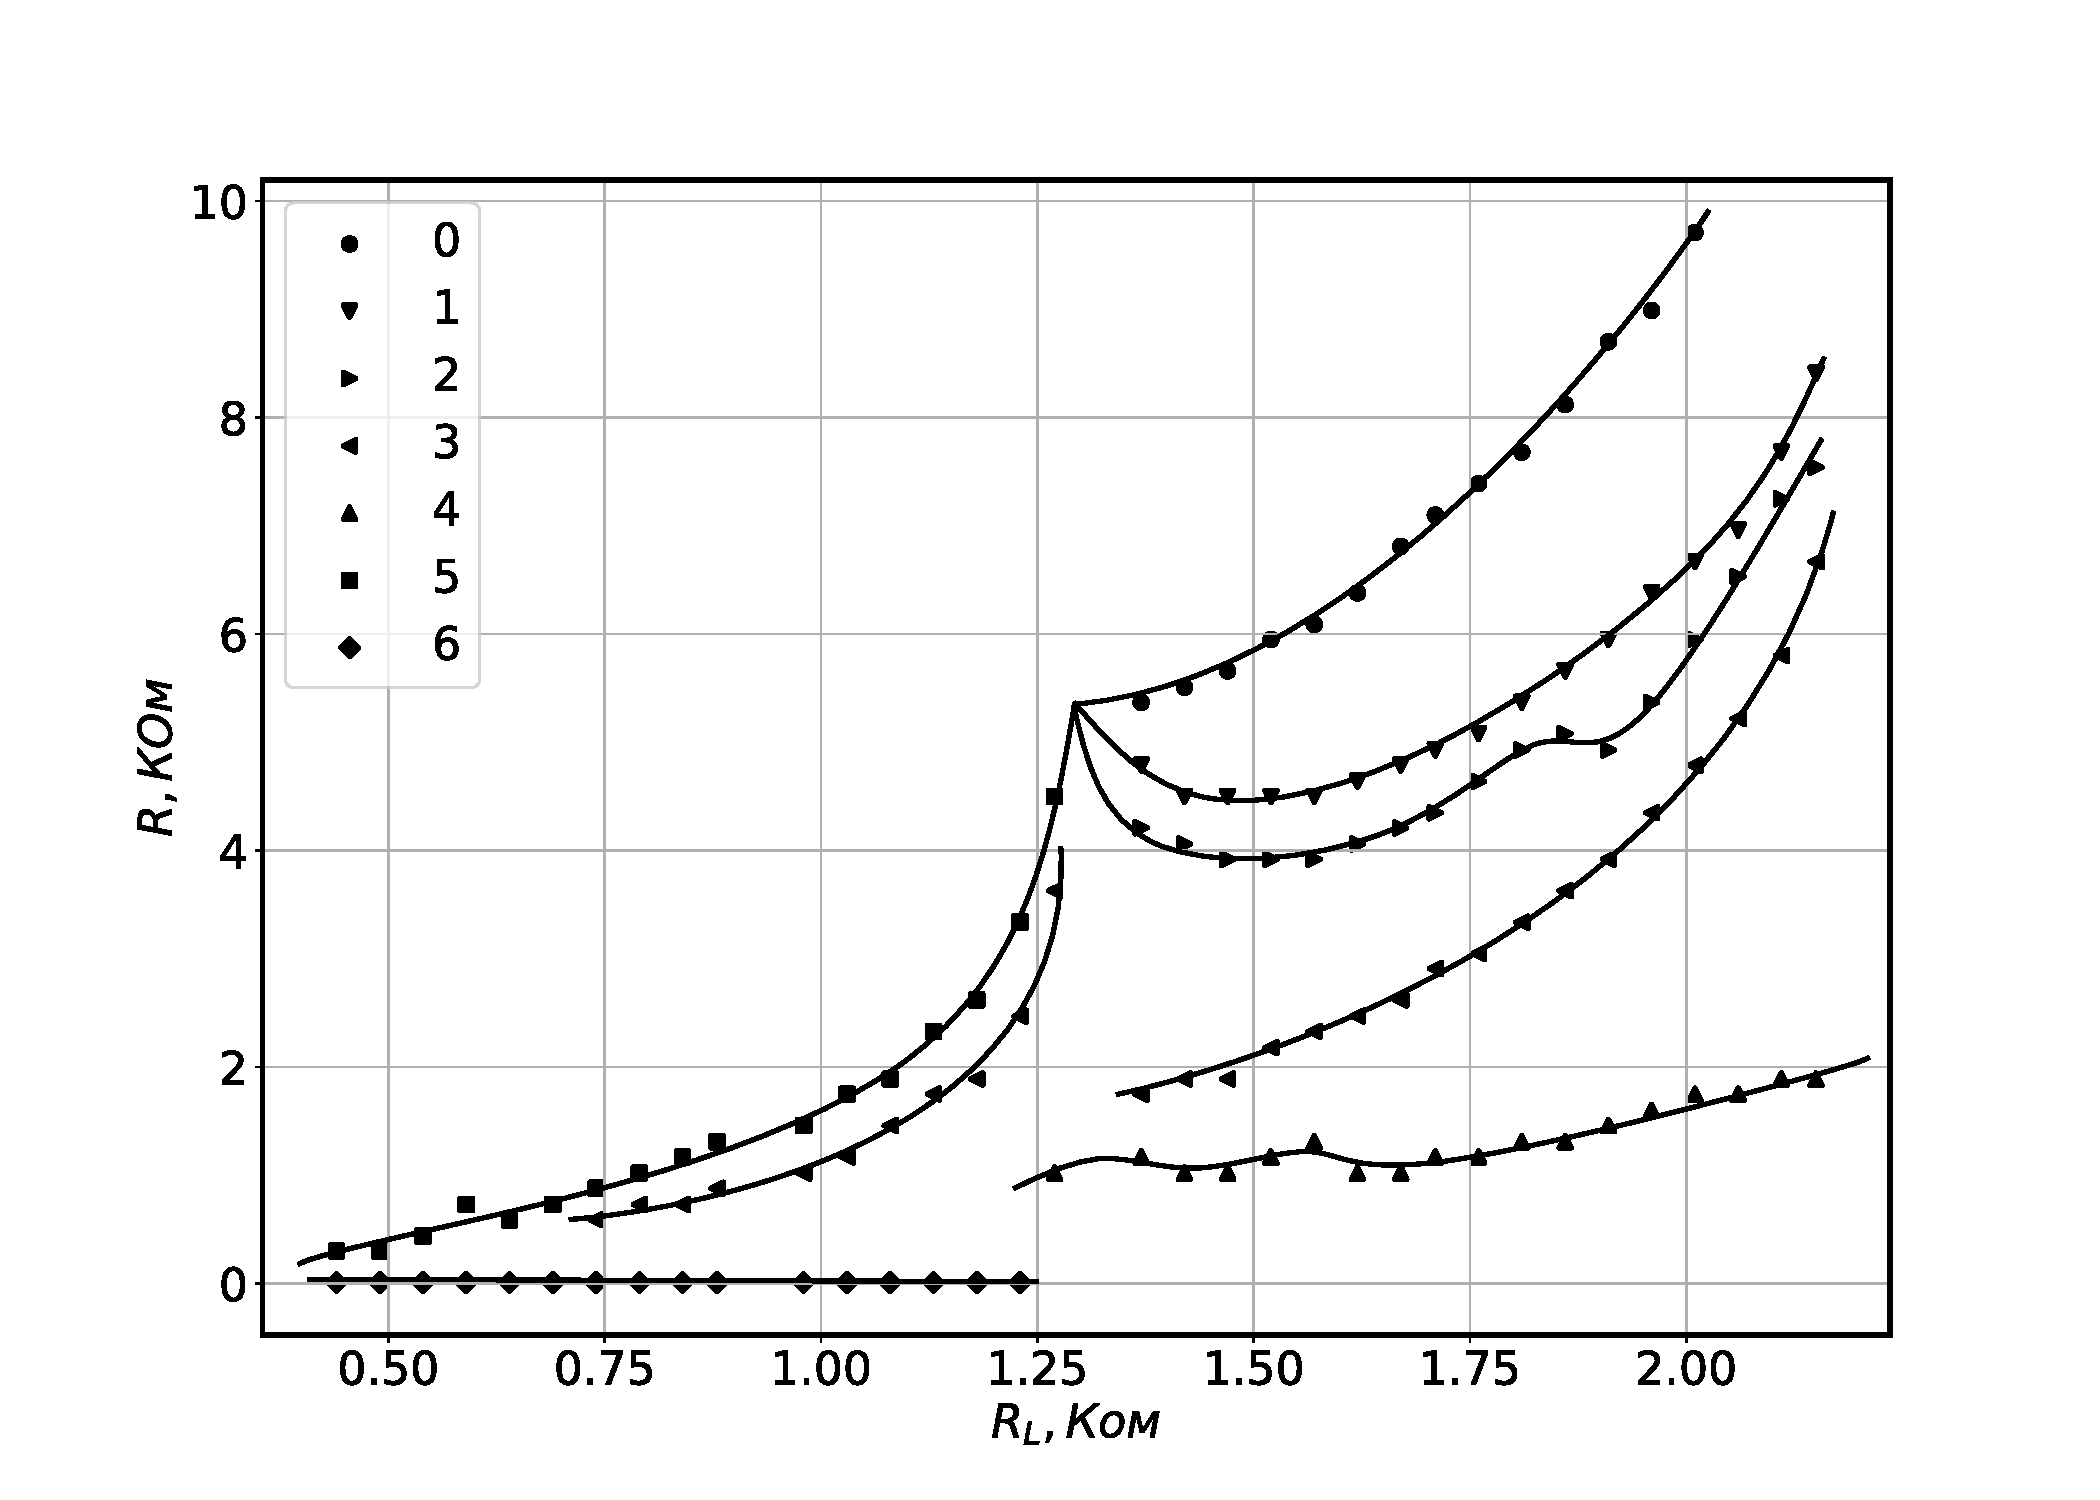
\includegraphics[width=0.75\textwidth]{bif_diag_teor.pdf}
	\caption{Диаграмма состояний системы при различных $R$ и $R_L$. 
	Цифрами обозначены граничные кривые для состояний: 
	0 --- большой предельный цикл и двухпетлевой аттрактор,
	1 --- двухпетлевой аттрактор и аттрактор Рёсслера,\
	2 --- аттрактор Рёсслера и малый предельный цикл,
	3 --- малый предельный цикл и фокус, 
	4 --- фокус и малый предельный цикл, 
	5 --- большой предельный цикл и малый предельный цикл,
	6 --- фокус и малый предельный цикл.}
	\label{fig:phase_diag_teor}
\end{figure}

\section*{Выводы}

\begin{thebibliography}{9}
	\bibitem{LabBook}
	Лабораторный практикум по общей физике, Том 2, под редакцией А. Д. Гладуна
\end{thebibliography}

\section*{Приложения}
\subsection*{Характеристики используемой схемы Чуа}
В качестве операционных усилителей были использованы TL082CP.
\begin{table}[H]
	\centering
	\begin{tabular}{|r|r|r|r|r|r|}
		\hline
		$R_1$ & $220$ Ом   & $R_6$  & $3.3$ КОм  & $R$   & $4.7$ КОм \\ \hline
		$R_2$ & $220$ Ом   & $R_7$  & $100$ Ом   & $C$   & $100$ нФ  \\ \hline
		$R_3$ & $2.2$ КОм  & $R_8$  & $3.3$ КОм  & $C_1$ & $10$ нФ   \\ \hline
		$R_4$ & $22.0$ КОм & $R_9$  & $1.0$ КОм  & $C_2$ & $100$ нФ  \\ \hline
		$R_5$ & $22.0$ КОм & $R_{10}$ & $10.0$ КОм &       &           \\ \hline
	\end{tabular}
	\caption{Характеристики используемых элементов.}
	\label{tab:curcuit_chars}
\end{table}
\end{document}